\documentclass[a4paper,ngerman]{scrartcl}

\usepackage{amsmath}
\usepackage{amsfonts}
\usepackage{amssymb}
\usepackage[utf8]{inputenc}
\usepackage{graphicx}
\usepackage[ngerman]{babel}
\usepackage{hyperref}
\usepackage{float}
\usepackage{caption}
\usepackage{subcaption}
\usepackage{multirow}  %for tables
\usepackage{icomma} % Handle german comma as decimal point in numbers
\usepackage{units,siunitx} % Write units with correct spacing
\usepackage{upgreek} % provide non-italic greek letters
\usepackage{url}
%\usepackage{subfig}

% Formatting of table & figure captions
\captionsetup{font={sf,footnotesize},labelfont=bf,textfont=sl,skip=6pt}
\setlength{\abovecaptionskip}{6pt}
\setlength{\belowcaptionskip}{0pt}

\title{Black Lipid Membrane}
\date{\today}
\author{Michel Rausch, Michael Eliachevitch}

\begin{document}

\maketitle
\tableofcontents
\newpage

\section{Einleitung}

In diesem Versuch werden Ionenkanäle in planaren Lipidmembranen untersucht. Hierbei wird der Wirkmechanismus des Antibiotikums Gramacidin A untersucht. In einer biologischen Zelle gelangen durch die entstandenen Kanäle Kationen durch die Zellmembran. Die Zelle stirbt aufgrund der Zerstörung ihres elektrochemischen Gradients [\ref{ref:mappe}].

Gramicidin beschreibt eine Gruppe Antibiotika. Dieses ist kommerziell unter Namen wie Angidin\textregistered , Mycolog\textregistered , Topsym\textregistered , Neospiron\textregistered  verfügbar. 


\section{Theoretische Grundlagen}

Die chemischen Grundlagen werden hier nicht genau behandelt. Gramicidin A1 besitzt die Summenformel $C_{99}H_{140}N_{20}O_{17}$. Es kann in der Natur von erdlebenden Bakterien beobachtet, aber auch synthetisch hergestellt werden. Mehrere Strukturen sind möglich, wobei Gramicidin A die häufigste ist. Gramicidin besitzt eine zyklische Struktur und damit einen anderen Wirkmechanismus. In diesem Experiment wird lediglich die Variante A verwendet.

\subsection{Wirkmechanismus}

Es existieren verschiedene Modelle, die Beschreiben, wie Gramicidin A (GA) in die Zellmembran integriert wird. Diese sind in Abbildung \ref{fig:wirkmechanismus} gezeigt.

\begin{figure}
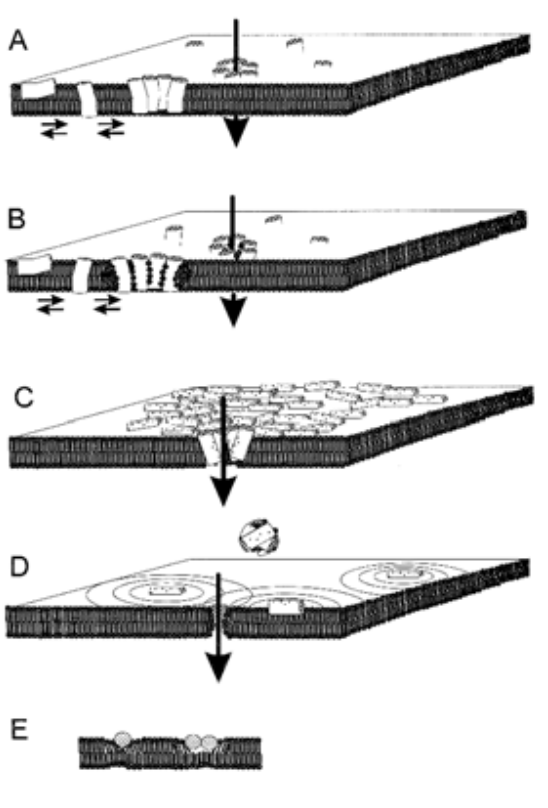
\includegraphics[width=0.6\textwidth]{wirkmechanismus.png}
\caption{Verschiedene Modelle zur Erklärung der Zerstörung einer Bakterienzelle mittels Peptid-Antibiotika [\ref{ref:mappe}]}
\label{fig:wirkmechanismus}
\end{figure}

\subsection{Ionentransport}
	

\subsubsection{Einzelkanaltransport}



\subsubsection{Mehrkanaltransport}


\subsubsection{Autokorrelationsfunkion}


\subsubsection{Charakteristik einer Membran}






\section{Versuchsaufbau}








\section{Aufgabenstellung und Versuchsdurchführung}










\section{Quellen}
\begin{enumerate}
\item Vorbereitungsmappe \label{ref:mappe}
\item pharmawiki.ch (16.11.2014) \label{ref:pharmawiki}
\end{enumerate}



\end{document}
